\documentclass[12pt,letterpaper,noanswers]{exam}
\usepackage[usenames,dvipsnames,svgnames,table]{xcolor}
\usepackage[margin=0.9in]{geometry}
\renewcommand{\familydefault}{\sfdefault}
\usepackage{multicol}
\pagestyle{head}
\header{AM 108 Class 32}{}{H\'enon map}
\runningheadrule
\headrule
\usepackage{graphicx} % more modern
\usepackage{amsmath} 
\usepackage{amssymb} 
\usepackage{hyperref}
\usepackage{tcolorbox}

\begin{document}
 \pdfpageheight 11in 
  \pdfpagewidth 8.5in

\noindent 




\begin{itemize}
\itemsep0em
\item You have a project weekly log due Friday (and again next Friday).  Your project work is replacing problem sets.
\item The project progress presentation slides are due Monday Nov 30th at 11am ET (see Canvas assignment for more info).
\item The Quiz 02 Follow Up is due today.  The retake, if assigned to you, is due Thurs Dec 3rd.  Request a different due date via private message on Piazza, if needed.
\item Skill Check C31 retake will be on Monday Nov 30th.  (Our next class meeting is Monday Nov 30th).
\end{itemize}

\hrule
\vspace{0.2cm}



\noindent\textbf{Teams}




\vspace{0.2cm}

\hrule
\vspace{0.2cm}


\noindent\textbf{Big picture}

We are looking at the H\'enon map today.

\vspace{0.2cm}
\hrule
\vspace{0.2cm}
\noindent\textbf{Collaboration review}

\vspace{0.2cm}
\hrule
\vspace{0.2cm}

\noindent\textbf{Presentations}


\vspace{0.2cm}
\hrule
\vspace{0.2cm}
Zeroth iterate of the map: a rectangle of initial conditions (on the left).  The first iterate of those points is on the right.

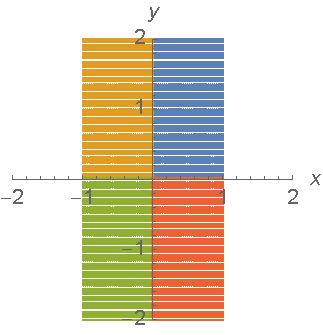
\includegraphics{img/20191125-p1a.pdf}
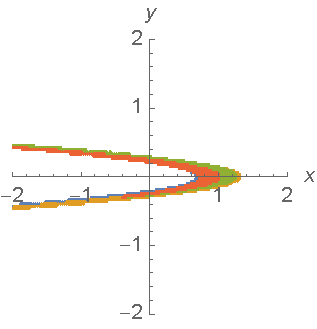
\includegraphics{img/20191125-p1b.pdf}

The second iterate is on the left and the third on the right.

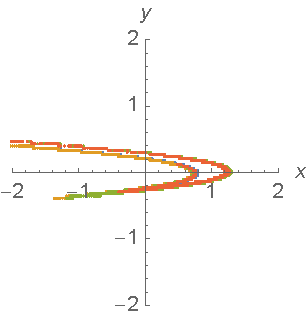
\includegraphics{img/20191125-p1c.pdf}
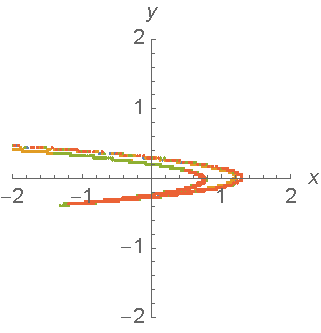
\includegraphics{img/20191125-p1d.pdf}

\vspace{0.2cm}
\hrule
\vspace{0.2cm}

\noindent\textbf{Your questions}
\begin{enumerate}
    \item Does the fact that the H\'enon map can be written as a composition of maps set the structure of its attractor?
    \item What is 'fractal microstructure'?
    \item Can we calculate ranges for $a$ and $b$ that will produce chaos?
    \item There is a $+1$ shift in the map.  How important is the $+1$ value?
    \item How do we determine whether an attractor is globally attracting?  (Is the attractor for the H\'enon map?)
    \item Are chaotic attractors and strange attractors the same thing?
    \item Is there a program for visualizing the structure of the Lorenz attractor?
    \item Steve writes that the H\'enon map attractor is `the closure of a branch of the unstable manifold' of a saddle point.  What does this mean?
\end{enumerate}

\vspace{0.2cm}
\hrule
\vspace{0.2cm}

\noindent\textbf{Skill Check C33 practice}
\begin{questions}
\item Skill check C31 retake.

\end{questions}

\vspace{0.2cm}

\hrule
\vspace{0.2cm}


\noindent\textbf{Questions}

\noindent \ \ 0.  Share a plant, tree, flower, etc that you like with your team, and write your names on the slide.

\begin{questions}
\item The H\'enon map is given by $x_{n+1} = 1 + y_n - a x_n^2$ and $y_{n+1} = b x_n$.  Consider the series of transformations
$T': x' = x, y' = 1 + y - a x^2$, 
$T'': x'' = b x', y'' = y'$, 
$T''': x''' = y'', y''' = x''.$  
\begin{figure}[h]
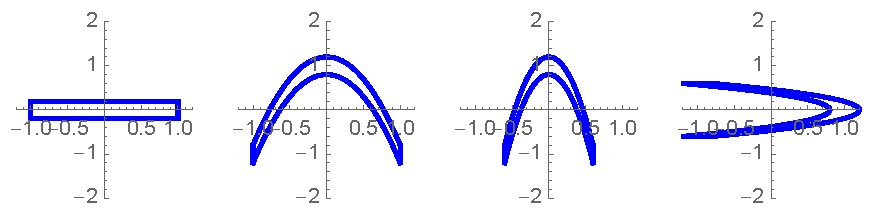
\includegraphics{img/C25Henon.pdf}
\caption{The transformations $T'$, $T''$ and $T'''$ are composed from left to right, with $T'$ operating on the rectangle on the far left.}
\end{figure}
\begin{parts}
\item (12.2.1) Show that composing this series ($T''' T'' T'$) of transformations yields the H\'enon map.
\item (12.2.2) Show that the transformations $T'$ and $T''$ are area preserving but $T''$ is not.

\textit{A vector calculus interlude: think of the map $T'$ as a coordinate transformation from coordinates $xy$ to coordinates $x'y'$.  
We are interested in the area of a region of the $xy$ plane after it undergoes the coordinate transformation.  Recall:
$\iint_R dx\ dy = \iint_S \left\vert \frac{\partial(x,y)}{\partial(x',y')}\right\vert dx'dy'$} where $ \frac{\partial(x,y)}{\partial(x',y')} =
\left\vert \begin{array}{ c c} \frac{\partial x}{\partial x'} & \frac{\partial x}{\partial y'} \\ \frac{\partial y}{\partial x'} & \frac{\partial y}{\partial y'} \end{array} \right\vert.$
\end{parts}

\item The H\'enon map is given by 
\begin{align*}
x_{n+1} = &\ 1 + y_n - a x_n^2 \\
y_{n+1} = &\ b x_n.
\end{align*}
\begin{parts}
\item (12.2.4) Find all of the fixed points of this map and give an existence condition for them.
\item (12.2.5) Calculate the Jacobian matrix of the Hénon map and find its eigenvalues.  
\item (12.2.6) A fixed point of a map is linearly stable if all eigenvalues satisfy $\vert \lambda \vert < 1$.  Consider $-1 <  b < 1$.

The fixed points are of the form $x = -c \pm \sqrt{c^2 + d}$.  The $ x = -c - \sqrt{c^2 + d}$ fixed point is always unstable.
Consider the $x = -c + \sqrt{c^2 + d}$ fixed point.  Using the contour plots below for the value of each eigenvalue, what is its stability?
\begin{figure}[h]
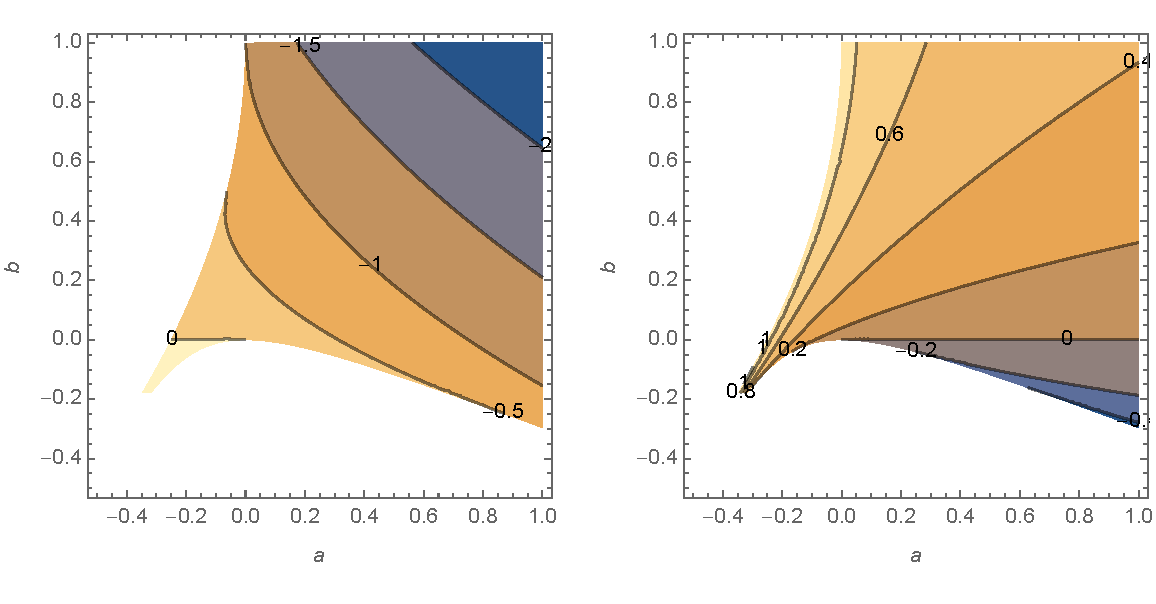
\includegraphics[scale=0.4]{img/C26henon2.pdf}
\end{figure}
% \item \textit{Come back to this if time permits, but skip ahead to the Smale horseshoe for now}.  
% Along the line $a = \frac{3}{4}(1-b)^2$, one of the eigenvalues attains $\lambda = -1$.
% Show that for $a>\frac{3}{4}(1-b)^2$, there is a 2-cycle.
\end{parts}
\end{questions}

Some answers:
\begin{enumerate}
\item For $T'$, $\left\vert \begin{array}{c c} 1 & 0 \\ -2 a x & 1 \end{array} \right\vert = 1$.  For $T''$, 
 $\left\vert \begin{array}{c c} b & 0 \\ 0 & 1 \end{array} \right\vert = b$.
 For $T'''$, $\left\vert \begin{array}{c c} 0 & 1 \\ 1 & 0 \end{array} \right\vert = \vert -1 \vert = 1.$

\item 
\begin{enumerate}
\item $x^* = \frac{-1+b}{2a} \pm \sqrt{\left(\frac{-1+b}{2a}\right)^2 +1}$, $y^* = bx^*$, $\left(\frac{-1+b}{2a}\right)^2 +1>0$.
\item $\lambda = -ax^* \pm \sqrt{(ax^*)^2+b}$
\item Stable until $\lambda_1$ crosses $-1$.  Then there is a flip bifurcation.
\end{enumerate}
\end{enumerate}

\eject

\begin{questions}
\item[(Extra)] (12.1.7) The Smale horseshoe map is illustrated in the figure below.  In this map, some of the points that start in the unit square
are mapped outside the square after an iteration of the map.
\begin{figure}[h]
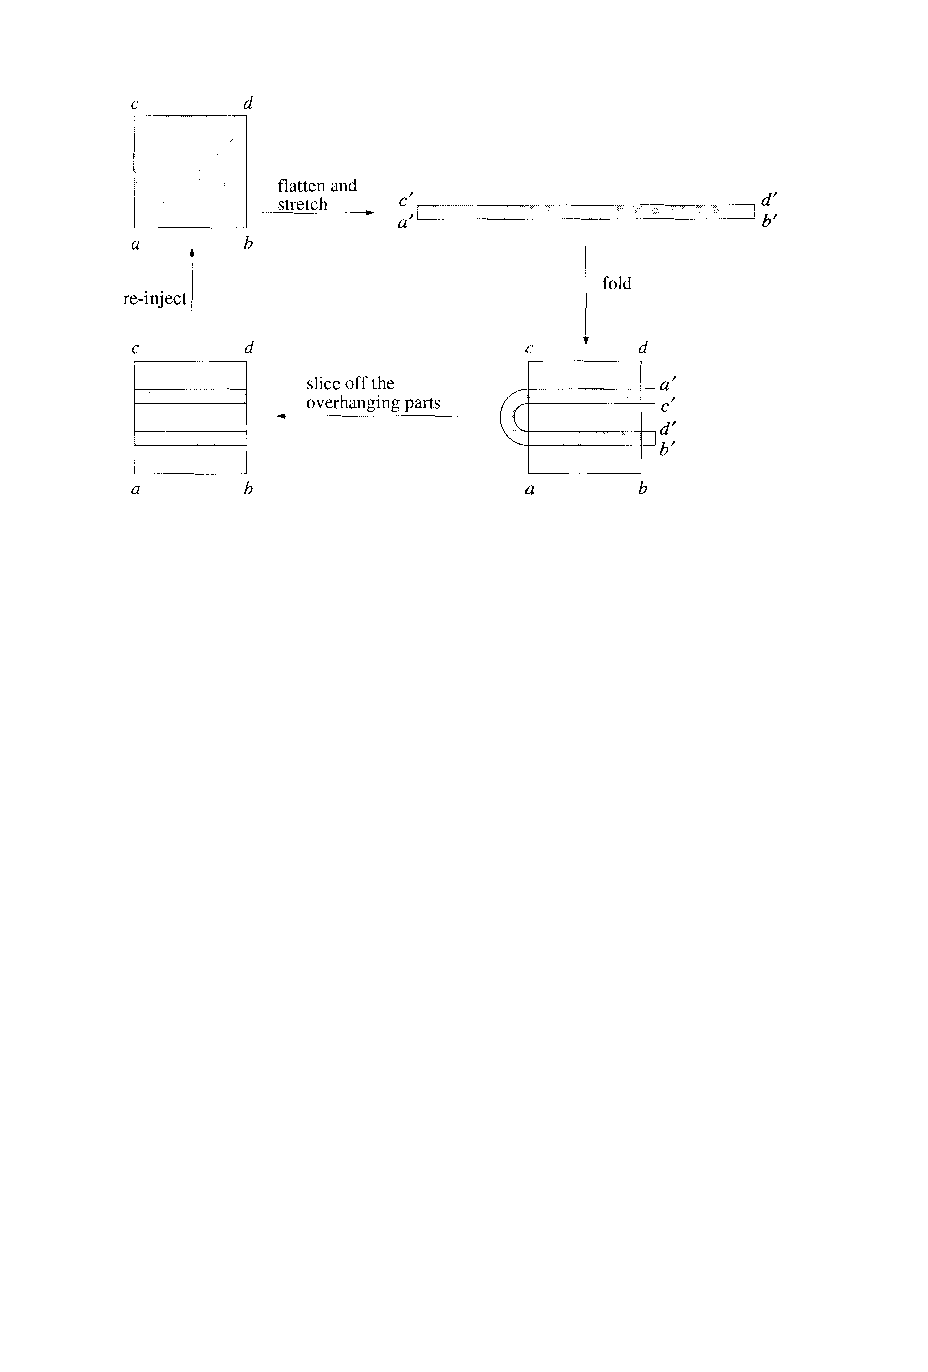
\includegraphics[scale=0.8]{img/C26smale2.pdf}
\caption{The Smale horseshoe map (from Strogatz)}
\end{figure}
\begin{parts}
\item In the original unit square, which regions remain in the unit square after one iteration?  Mark these regions $V_0$ and $V_1$.
\item Sketch the effect of a second iteration of the map.  Identify the points in the original unit square that survived two iterations.
Mark these regions $V_{00}, V_{01}, V_{10}, V_{11}$.
\item Work to identify the set of points in the original unit square that survive forever under forward iterations of the map.
\item Now consider a backward iterate of the map.  
Which points stay in the unit square under a backward iteration?  Mark these regions $H_{0}$ and $H_1$
\item What about under two backward iterations?  Mark these regions $H_{00}$, etc.
\item Attempt to construct the set of points that is in the unit square for all time (both forward and backward).
%\item Add horizontal lines to the unit square on the right.  Use these to find the regions
% $H_{10} = H_1\cap f(H_0)$, $H_{00} = H_0\cap f(H_0)$, etc.
% \item Now run the map forward again.  Some points from the original square survive two iterates.  Where are these points
% located in the original square?
% \item 
\end{parts}
\end{questions}

\noindent Some answers: 
\begin{enumerate}
\item[(Extra)]
\begin{enumerate}
\item  In the map, the pieces that return to the unit square correspond to a chunk towards the left and a chunk towards the right
of the thin flattened, stretched, bar.  Stepping back to the initial square, these chunks correspond to vertical stripes.
\item For the second iterate, we stretch the segmented unit square and the 2 horizontal lines stretch to the entire length of the stretched
and flattened intermediate step.  These are then bent around and put into the square, so we have four thin lines, in two pairs 
\end{enumerate}
\end{enumerate}
\end{document}